
%(BEGIN_QUESTION)
% Copyright 2006, Tony R. Kuphaldt, released under the Creative Commons Attribution License (v 1.0)
% This means you may do almost anything with this work of mine, so long as you give me proper credit

Match these component names with parts in this valve illustration (note the arrows):

\begin{itemize}
\item{} Bonnet
\item{} Seat
\item{} Stem
\item{} Plug
\item{} Packing
\item{} Pipe flange
\item{} Body
\item{} Bushing
\item{} Packing flange (or packing gland)
\end{itemize}

$$\includegraphics[width=15.5cm]{i00771x01.eps}$$

Also, explain why the direction of flow shown in this illustration goes from left to right.  What would happen if we sent fluid flow through this valve from right to left instead?

\underbar{file i00771}
%(END_QUESTION)





%(BEGIN_ANSWER)

$$\includegraphics[width=15.5cm]{i00771x02.eps}$$

If we were to use this valve ``backwards,'' the pressure drop across the plug would tend to ``slam'' it closed whenever it approached the closed position.  In other words, the process fluid's differential pressure drop would make it very difficult to maintain any plug position near full-closed.

This is actually an example of a mechanical feedback system.  As the valve closes, the pressure drop across it (in most processes) usually rises because other pressure losses in the piping system decrease with decreased flow, leaving the valve to drop all the fluid pressure.  Since plug position has an effect on pressure drop, and pressure drop exerts a mechanical force on the plug, there is a system of feedback at work here.

In the proper flow direction, the feedback is negative: closing the valve results in greater pressure drop, which in turn tries to keep the valve open.  In true negative feedback form, the feedback works {\it against} the initial action.  The more the valve is closed, the more the process pressure tries to keep it open.

In the backwards flow direction, the feedback is positive: closing the valve results in greater pressure drop, which in turn tries to close the valve even more.  The result is a tendency for the system to {\it saturate}, staying open or slamming shut, but avoiding any in-between conditions.  This makes it very difficult to position the valve mechanism near full-closed, and would result in erratic control near the lower end of the valve's working range.


%(END_ANSWER)





%(BEGIN_NOTES)


%INDEX% Final Control Elements, valve: globe valve component identification

%(END_NOTES)


